\chapter{嵌入式系统中的I/O接口驱动}{驱动}

\section{实验目的}
\begin{itemize}\itemsep=-3pt
  \item 学习嵌入式Linux操作系统设备驱动的方法;
\end{itemize}

\section{接口电路介绍}
	Linux以模块的形式加载设备类型, 通常一个模块对应一个设备驱动, 因此是可以
分类的.将模块分成不同的类型并不是一成不变的, 开发人员可以根据实际工作需要
在一个模块中实现不同的驱动程序.一般情况, 一个设备驱动对应一类设备的模块方式, 
这样便于多个设备的协调工作, 也利于应用程序的开发和扩展.

	设备驱动程序负责将应用程序如读、写等操作正确无误的传递给相关的硬件, 并使
硬件能够做出正确反应.因此在编写设备驱动程序时, 必须要了解相应的硬件设备的
寄存器、IO口及内存的配置参数.

	设备驱动在准备好以后可以编译到内核中, 在系统启动时和内核一起启动, 这种
方法在嵌入式~Linux~系统中经常被采用.在开发阶段, 设备驱动的动态加载更为普遍.
开发人员不必在调试过程中频繁启动机器就能完成设备驱动的调试工作.

	嵌入式处理器片内集成了大量的可编程设备接口, 为构成处理器系统带来了极大的
便利.S5PV210 有 237 只多功能引脚, 大多数是功能复用的, 可以通过初始化编程
将它们设置为GPIO(General Purpose I/O, 通用IO)或者某个具体功能.本章实验通过
学习 GPIO 对一些设备的控制, 掌握Linux设备驱动的基本方法.

\subsection{LED}
\begin{figure}
\centering
\subfloat[LED控制信号]{
  \label{led4}
  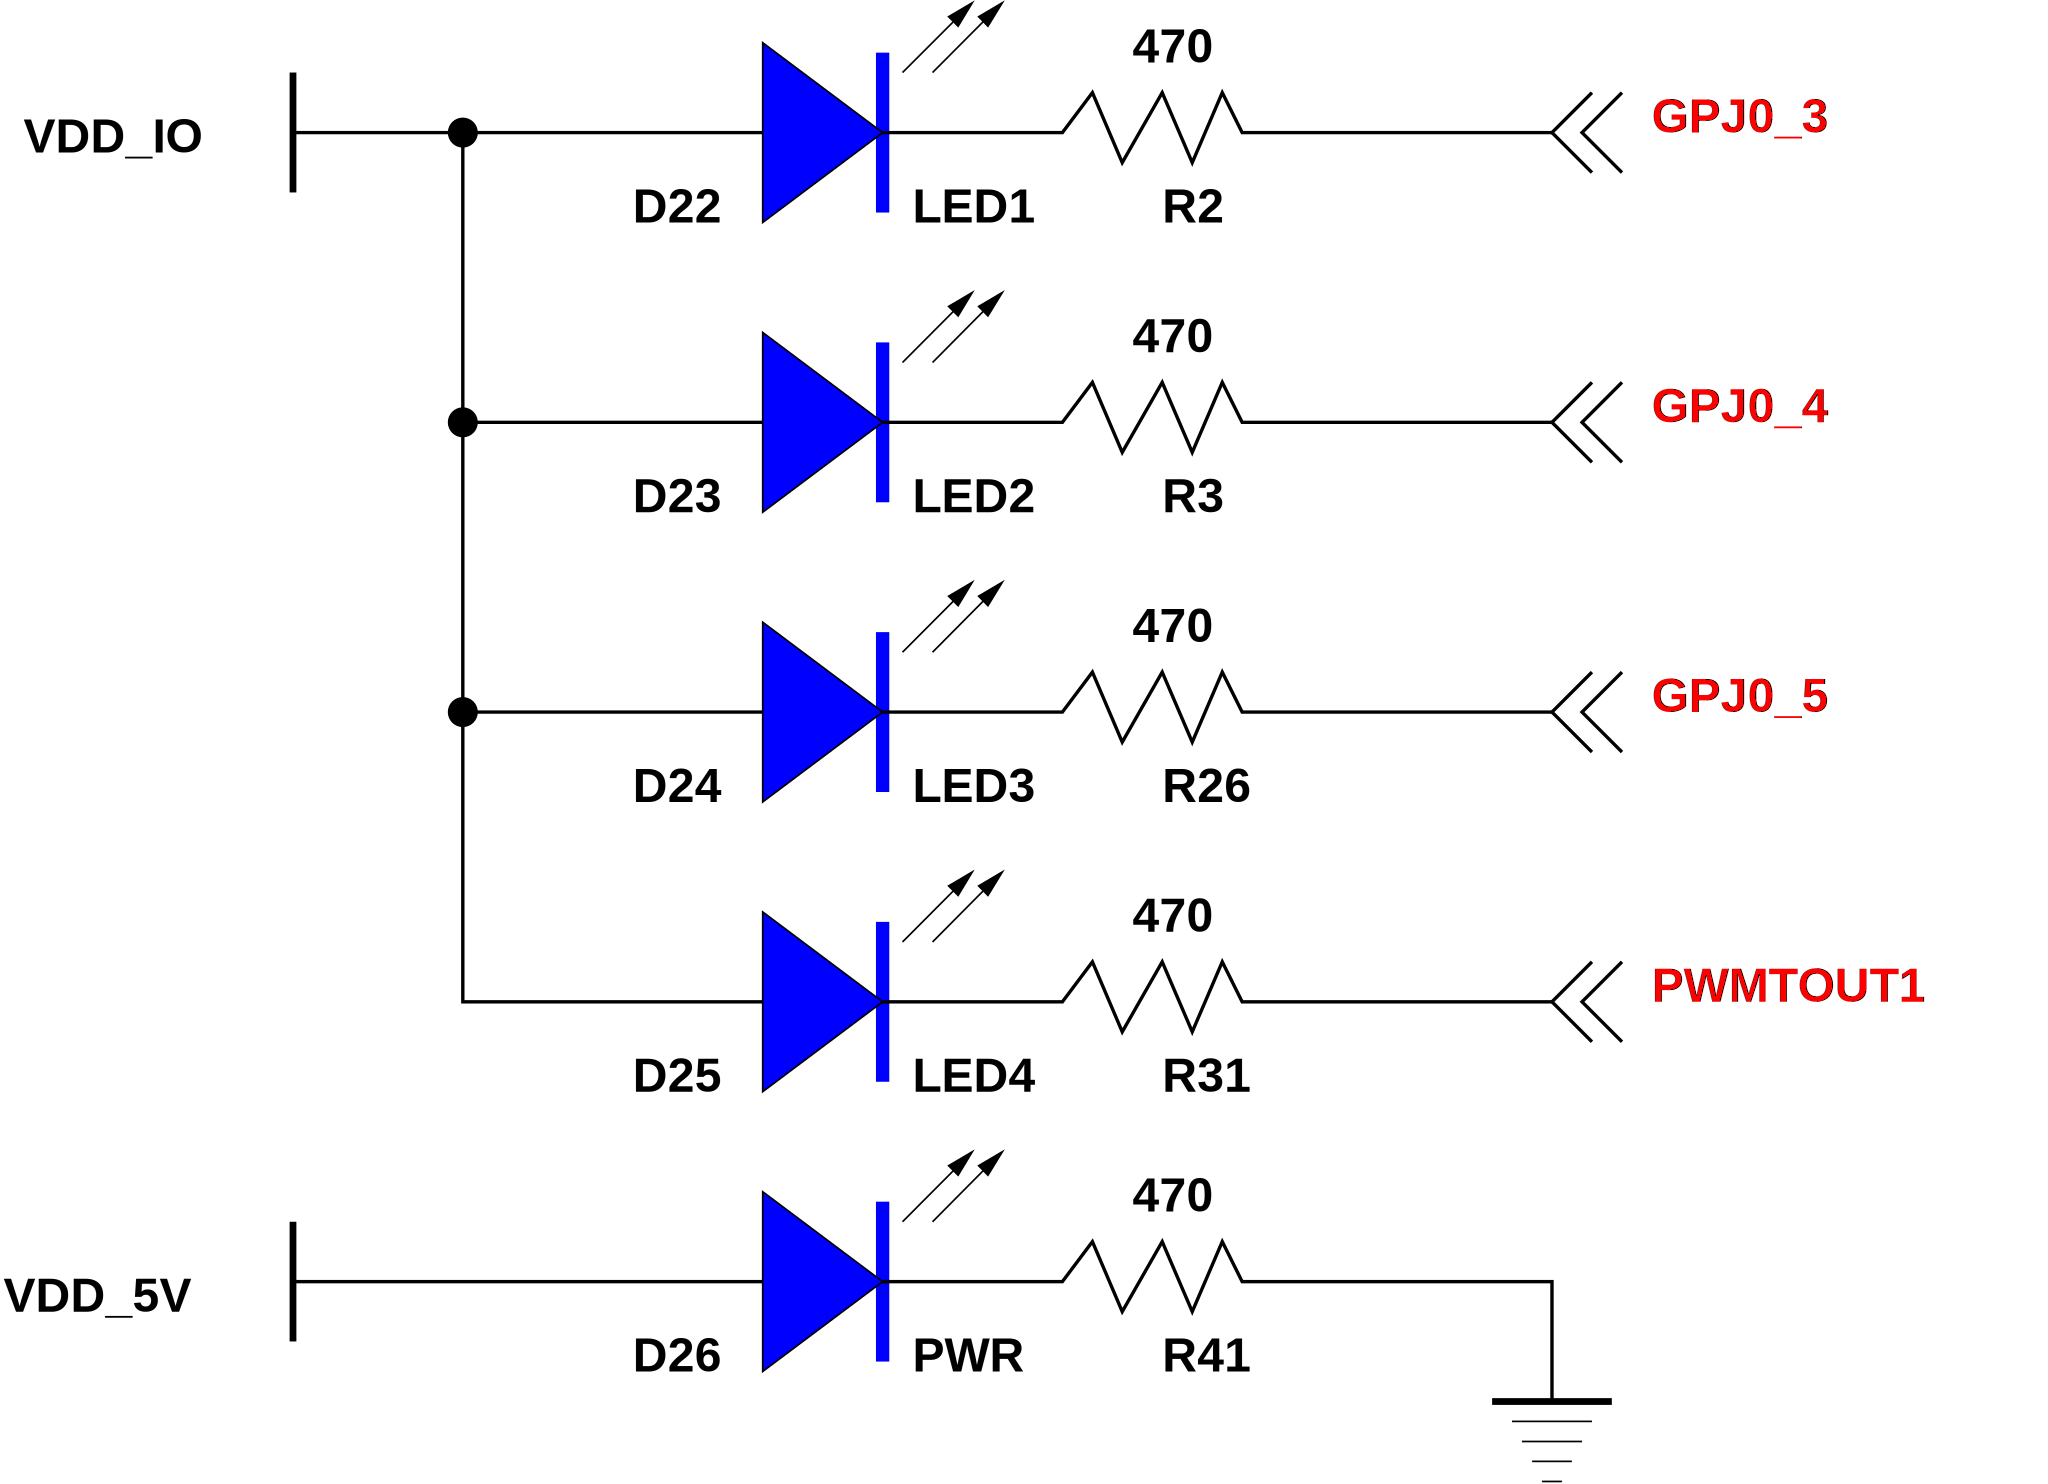
\includegraphics[width=.4\textwidth]{led4}
}\hspace{5mm}
\subfloat[按键控制信号]{
  \label{keypad}
  \includegraphics[width=.3\textwidth]{keypad}
}
\caption{简单的I/O设备}\label{simple_IO}
\end{figure}

	本系统有 5 个LED, 其中一个是电源指示, 三个通过 GPJ0 的三只引脚控制,
一个通过PWMTOUT1控制.结构图如\ref{led4}.

	通过GPIO控制LED, 还需要了解系统的硬件资源分配.表{}\ref{regs1} 列出了
GPJ0的相关寄存器, 寄存器的功能含义在表{}\ref{regs2}中.
	
\begin{table}[!h]
\centering
\caption{GPJ0 寄存器地址}\label{regs1} \ \\

\begin{tabular}{|l|c|l|}
\hline
\multicolumn{1}{|c|}{寄存器名} & 地址 & 
\multicolumn{1}{c|}{描述} \\\hline
	GPJ0CON   & 0xE020\_0240 & GPJ0 配置寄存器              \\\hline
	GPJ0DAT   & 0xE020\_0244 & GPJ0 数据寄存器              \\\hline
	GPJ0PUD   & 0xE020\_0248 & GPJ0 上拉/下拉寄存器         \\\hline
	GPJ0DRV   & 0xE020\_024C & GPJ0 驱动强度控制寄存器      \\\hline
	GPJ0CONPDN& 0xE020\_0250 & GPJ0 掉电模式配置寄存器      \\\hline
	GPJ0PUDPDN& 0xE020\_0254 & GPJ0 掉电模式上拉/下拉寄存器 \\\hline
\end{tabular}
\end{table}


\begin{center}
\longtable{|l|c|l|}
\caption{寄存器描述}\label{regs2}\\
\hline
\multicolumn{1}{|c|}{寄存器} & 位域 & \multicolumn{1}{c|}{描述} \\\thline
\endfirsthead
\caption{寄存器描述(续)}\\
\hline
\multicolumn{1}{|c|}{寄存器} & 位域 & \multicolumn{1}{c|}{描述} \\\thline
\endhead
\hline \endfoot
\endlastfoot
    GPJ0CON[7] & [31:28] & 0000 = Input                 \\
               &         & 0001 = Output                \\
               &         & 0010 = MSM\_ADDR[7]          \\
               &         & 0011 = CAM\_B\_DATA[7]       \\
               &         & 0100 = CF\_DMACKNs           \\
               &         & 0101 = MHL\_D0               \\
               &         & 0110 $\sim$ 1110 = Reserved  \\
               &         & 1111 = GPJ0\_INT[7]          \\\hline
    GPJ0CON[6] & [27:24] & 0000 = Input                 \\
               &         & 0001 = Output                \\
               &         & 0010 = MSM\_ADDR[6]          \\
               &         & 0011 = CAM\_B\_DATA[6]       \\
               &         & 0100 = CF\_DRESETN           \\
               &         & 0101 = TS\_ERROR             \\
               &         & 0110 $\sim$ 1110 = Reserved  \\
               &         & 1111 = GPJ0\_INT[6]          \\\hline
    GPJ0CON[5] & [23:20] & 0000 = Input                 \\
               &         & 0001 = Output                \\
               &         & 0010 = MSM\_ADDR[5]          \\
               &         & 0011 = CAM\_B\_DATA[5]       \\
               &         & 0100 = CF\_DMARQ             \\
               &         & 0101 = TS\_DATA              \\
               &         & 0110 $\sim$ 1110 = Reserved  \\
               &         & 1111 = GPJ0\_INT[5]          \\\hline
    GPJ0CON[4] & [19:16] & 0000 = Input                 \\
               &         & 0001 = Output                \\
               &         & 0010 = MSM\_ADDR[4]          \\
               &         & 0011 = CAM\_B\_DATA[4]       \\
               &         & 0100 = CF\_INTRQ             \\
               &         & 0101 = TS\_VAL               \\
               &         & 0110 $\sim$ 1110 = Reserved  \\
               &         & 1111 = GPJ0\_INT[4]          \\\hline
    GPJ0CON[3] & [15:12] & 0000 = Input                 \\
               &         & 0001 = Output                \\
               &         & 0010 = MSM\_ADDR[3]          \\
               &         & 0011 = CAM\_B\_DATA[3]       \\
               &         & 0100 = CF\_IORDY             \\
               &         & 0101 = TS\_SYNC              \\
               &         & 0110 $\sim$ 1110 = Reserved  \\
               &         & 1111 = GPJ0\_INT[3]          \\\hline
    GPJ0CON[2] & [11:8]  & 0000 = Input                 \\
               &         & 0001 = Output                \\
               &         & 0010 = MSM\_ADDR[2]          \\
               &         & 0011 = CAM\_B\_DATA[2]       \\
               &         & 0100 = CF\_ADDR[2]           \\
               &         & 0101 = TS\_CLK               \\
               &         & 0110 $\sim$ 1110 = Reserved  \\
               &         & 1111 = GPJ0\_INT[2]          \\\hline
    GPJ0CON[1] &  [7:4]  & 0000 = Input                 \\
               &         & 0001 = Output                \\
               &         & 0010 = MSM\_ADDR[1]          \\
               &         & 0011 = CAM\_B\_DATA[1]       \\
               &         & 0100 = CF\_ADDR[1]           \\
               &         & 0101 = MIPI\_ESC\_CLK        \\
               &         & 0110 $\sim$ 1110 = Reserved  \\
               &         & 1111 = GPJ0\_INT[1]          \\\hline
    GPJ0CON[0] &  [3:0]  & 0000 = Input                 \\
               &         & 0001 = Output                \\
               &         & 0010 = MSM\_ADDR[0]          \\
               &         & 0011 = CAM\_B\_DATA[0]       \\
               &         & 0100 = CF\_ADDR[0]           \\
               &         & 0101 = MIPI\_BYTE\_CLK       \\
               &         & 0110 $\sim$ 1110 = Reserved  \\
               &         & 1111 = GPJ0\_INT[0           \\\hline
    GPJ0DAT    &  [7:0]  & 端口配置为输入时, 从寄存器读入值对应位反映引脚电平\\
               &         & 状态; 端口配置为 输出时, 写出位产生对应引脚电平; \\
               &         & 端口配置为功能引脚时, 寄存器值不确定 \\\hline
    GPJ0DRV[n] &  [2n+1:2n] & 00 = 1$\times$             \\
               & n=0$\sim$7 & 01 = 2$\times$             \\
               &            & 10 = 3$\times$             \\
               &            & 11 = 4$\times$             \\\hline
    GPJ0CONPDN[n] &  [2n+1:2n] & 00 = 输出 0           \\
                  & n=0$\sim$7 & 01 = 输出 1           \\
                  &            & 10 = 输入             \\
                  &            & 11 = [保留]           \\\hline
    GPJ0PUDPDN[n] &  [2n+1:2n] & 00 = 禁止上拉/下拉    \\
                  & n=0$\sim$7 & 01 = 下拉             \\
                  &            & 10 = 上拉             \\
                  &            & 11 = [保留]           \\\hline


\endlongtable
\end{center}

\subsection{I/O端口地址映射}
	RISC处理器(如ARM、PowerPC等)通常只实现一个物理地址空间, 外设I/O端口成为
内存的一部分.此时, CPU可以像访问一个内存单元那样访问外设I/O端口, 而不需要
设立专门的外设I/O指令.这两者在硬件实现上的差异对于软件来说是完全透明的, 
驱动程序开发人员可以将存储器映射方式的I/O端口和外设内存统一看作是``I/O内存''
资源.

	I/O设备的物理地址是已知的, 由硬件设计决定.但是~CPU~通常并没有为这些
已知的外设I/O内存资源的物理地址预定义虚拟地址范围, 驱动程序不能直接通过物理
地址访问I/O设备, 而必须通过页表将它们映射到内核虚地址空间, 然后才能根据映射
所得到的内核虚地址范围, 通过访内指令访问这些I/O设备.~Linux~的内核函数
~ioremap()~ 用来将I/O设备的物理地址映射到内核虚地址空间.其原型如下:

	void * ioremap(unsigned long phys\_addr, unsigned long size, unsigned long
flags)

	端口释放时, 应通过函数iounmap()取消ioremap()所做的映射:

	void iounmap(void * addr)

	当I/O设备的物理地址被映射到内核虚拟地址后, 就可以像读写 RAM 那样直接读写
I/O设备资源了.例如可以通过下面的方式点亮最左边的一个LED:

\begin{boxedminipage}{.9\textwidth}
\lstset{language=c,escapeinside=``}
%\lstset{backgroundcolor=\color{bg}}
\begin{lstlisting}{}
#define	GPJ0CON		0xE0200240
#define	GPJ0DAT		0xE0200244
......

  `/* 映射控制寄存器地址 */`
  volatile int *pConfReg = ioremap(GPJ0CON, 4);
  `/* 映射数据寄存器地址 */`
  volatile int *pDataReg = ioremap(GPJ0DAT, 4);

  *pConfReg &= 0xFFFF0FFF;           `/* 只改变GPJ0\_3设置   */`
  *pConfReg |= 0x00001000;           `/* GPJ0\_3 设为输出    */`

  *pDataReg &= ~(1 << 3);            `/* GPJ0\_3 输出低电平  */`
......
\end{lstlisting}
\end{boxedminipage}
	
	为了保证驱动程序的跨平台的可移植性, 建议使用~Linux~中特定的函数来访问
~I/O~内存资源, 如~readb()、~readw()、~writeb()、~writew()~等.在RISC处理器里, 
它们实际上就是对存储器读写的重定义:

\begin{boxedminipage}{.9\textwidth}
\begin{verbatim}
#define readb(addr)  (*(volatile unsigned char *)__io_virt(addr))
#define readw(addr) (*(volatile unsigned short *)__io_virt(addr))
#define readl(addr) (*(volatile unsigned int *)__io_virt(addr))

#define writeb(b,addr) (*(volatile unsigned char *)__io_virt(addr) = (b))
#define writew(b,addr) (*(volatile unsigned short *)__io_virt(addr) = (b))
#define writel(b,addr) (*(volatile unsigned int *)__io_virt(addr) = (b))

......
\end{verbatim}
\end{boxedminipage}

\subsection{Key pad}
	S5PV210 内部设计了矩阵键盘接口, 但在我们的实验系统中, 只引出了少数的
按键开关, 这些按键都通过GPIO按位进行简单操作.在嵌入式系统中, 复杂的人机交互
可以通过更先进的设备(例如触摸屏等)完成.
按键开关逻辑结构如图\ref{keypad}.其中 KP\_COL0在GPIO的 GPJ1 组, KP\_COL1、
KP\_COL2、KP\_COL3 在GPJ2 组, EINT2 和 EINT3 在GPH0 组.EINT2和EINT3可以实现
外部中断.

	请根据数据手册, 设计实现按键的设备驱动.

\subsection{PWM 定时器}
	S5PV210内部有五个32位PWM定时器, 其中 Timer0、1、2、3 四个定时器可以输出
驱动PWM引脚.定时器时钟源来自APB-CLOCK, Timer0、1 共用一个 8 位预定标器,
Timer2、3、4 共用另一个 8 位定标器, 作为第一级分频;每个定时器还有各自的
除法器(分频数1、2 、4 、8 、16)作为第二级分频.

	每个定时器有一个32位的减法计数器, 由定时器计数寄存器TCNTBn载入初值.该值
减到零时向CPU产生中断, 并自动从TCNTBn重载, 进入下一轮循环, 除非定时器
控制寄存器 TCONn 中的定时器允许位被清除.清除 TCONn 的允许位导致定时器停止
工作, 计数器不再重载.

	PWM方式使用定时器比较寄存器 TCMPBn.当递减计数器的值与 TCMPBn 相匹配时, 
定时器输出电平发生改变, 因此, 比较寄存器决定了占空比.

	TCNTBn 和 TCMPBn 是双缓冲的, 允许在计数过程中更新, 更新值在下一个计数周期
生效.

	表\ref{timer_map}列出了与定时器相关的控制寄存器地址.定时器输入时钟

$$ CLOCK_{PWM} = \frac{PCLK}{(prescaler+1)*divider} $$

第一级分频系数 prescaler 来自 TCFG0:

	TCFG0[15:8] = prescaler1, 用于 Timer2、3、4;

	TCFG0[7:0] = prescaler0, 用于 Timer0、1;

	第二级分频数 ``divider value''由 TCFG1 中的 MUXn 提供:

\begin{center}
\begin{tabular}{|c|c|c|c|c|c|c|}
\hline
  [31:24] & [23:20] & [19:16] & [15:12] & [11:8] & [7:4] & [3:0] \\\hline
  Reserved & N/A & MUX4 & MUX3 & MUX2 & MUX1 & MUX0 \\\hline
\end{tabular}
 \ \\ \ \\

\begin{tabular}{|c|c|c|c|c|c|c|}
\hline
    MUX &  0000 & 0001 & 0010 & 0011 & 0100 & 0101 \\\hline
	分频/开关 &1/1 & 1/2 & 1/4 & 1/8 & 1/16 & SCLK\_PWM \\\hline
\end{tabular}
\end{center}

\begin{center}
\longtable{|l|c|l|}
\caption{定时器相关寄存器地址}\label{timer_map}\\
\hline
\multicolumn{1}{|c|}{寄存器名} & 地址 & \multicolumn{1}{c|}{描述} \\\hline
\endfirsthead
\caption{定时器相关寄存器地址(续)}\\
\hline
\multicolumn{1}{|c|}{寄存器名} & 地址 & \multicolumn{1}{c|}{描述} \\\hline
\endhead
\hline \endfoot
\endlastfoot
    TCFG0  & 0xE250\_0000 & 定时器配置寄存器1(2个 8-bit 预定标器)\\\hline
    TCFG1  & 0xE250\_0004 & 定时器配置寄存器2(5个二级分频选择开关)\\\hline
    TCON   & 0xE250\_0008 & 定时器控制寄存器\\\hline
    TCNTB0 & 0xE250\_000C & Timer 0 计数缓冲寄存器\\\hline
    TCMPB0 & 0xE250\_0010 & Timer 0 比较缓冲寄存器\\\hline
    TCNTO0 & 0xE250\_0014 & Timer 0 计数器观察寄存器\\\hline
    TCNTB1 & 0xE250\_0018 & Timer 1 计数缓冲寄存器\\\hline
    TCMPB1 & 0xE250\_001C & Timer 1 比较缓冲寄存器\\\hline
    TCNTO1 & 0xE250\_0020 & Timer 1 计数器观察寄存器\\\hline
    TCNTB2 & 0xE250\_0024 & Timer 2 计数缓冲寄存器\\\hline
    TCMPB2 & 0xE250\_0028 & Timer 2 比较缓冲寄存器\\\hline
    TCNTO2 & 0xE250\_002C & Timer 2 计数器观察寄存器\\\hline
    TCNTB3 & 0xE250\_0030 & Timer 3 计数缓冲寄存器\\\hline
    TCMPB3 & 0xE250\_0034 & Timer 3 比较缓冲寄存器\\\hline
    TCNTO3 & 0xE250\_0038 & Timer 3 计数器观察寄存器\\\hline
    TCNTB4 & 0xE250\_003C & Timer 4 计数缓冲寄存器\\\hline
    TCNTO4 & 0xE250\_0040 & Timer 4 计数器观察寄存器\\\hline
\endlongtable
\end{center}

	控制寄存器 TCON 用于5个定时器的工作方式设置.

\begin{center}
\longtable{|l|c|l|}
\caption{定时器控制寄存器}\\
\hline
\multicolumn{1}{|c|}{TCON} & 位域 & \multicolumn{1}{c|}{描述} \\\hline
\endfirsthead
\caption{定时器控制寄存器(续)}\\
\hline
\multicolumn{1}{|c|}{TCON} & 位域 & \multicolumn{1}{c|}{描述} \\\hline
\endhead
\hline \endfoot
\endlastfoot
  Reserved & [31:23]   & ---                               \\\hline
  Timer 4 自动重载     & [22] & 0 = 单次                   \\
                       &      & 1 = 自动重载               \\\hline
  Timer 4 手动更新     & [21] & 0 = 无操作                 \\
                       &      & 1 = 更新 TCNTB4            \\\hline
  Timer 4 启动/停止    & [20] & 0 = 停止                   \\
                       &      & 1 = 启动 Timer4            \\\hline
  Timer 3 自动重载     & [19] & 0 = 单次                   \\
                       &      & 1 = 自动重载               \\\hline
  Timer 3 输出反转开关 & [18] & 0 = 不反转                 \\
                       &      & 1 = TOUT\_3 反转           \\\hline
  Timer 3 手动更新     & [17] & 0 = 无动作                 \\
                       &      & 1 = 更新 TCNTB3            \\\hline
  Timer 3 启动/停止    & [16] & 0 = 停止                   \\
                       &      & 1 = 启动 Timer 3           \\\hline
  Timer 2 自动重载     & [15] & 0 = 单次                   \\
                       &      & 1 = 自动重载               \\\hline
  Timer 2 输出反转开关 & [14] & 0 = 不反转                 \\
                       &      & 1 = TOUT\_2 反转           \\\hline
  Timer 2 手动更新     & [13] & 0 = 无动作                 \\
                       &      & 1 = 更新 TCNTB2,TCMPB2     \\\hline
  Timer 2 启动/停止    & [12] & 0 = 停止                   \\
                       &      & 1 = 启动 Timer 2           \\\hline
  Timer 1 自动重载     & [11] & 0 = 单次                   \\
                       &      & 1 = 自动重载               \\\hline
  Timer 1 输出反转开关 & [10] & 0 = 不反转                 \\
                       &      & 1 = TOUT\_1 反转           \\\hline
  Timer 1 手动更新     & [9]  & 0 = 无动作                 \\
                       &      & 1 = 更新 TCNTB1,TCMPB1     \\\hline
  Timer 1 启动/停止    & [8]  & 0 = 停止                   \\
                       &      & 1 = 启动 Timer 1           \\\hline
  Reserved             & [7:5]&                            \\\hline
  死区允许/禁止        & [4]  &                            \\\hline
  Timer 0 自动重载     & [3]  & 0 = 单次                   \\
                       &      & 1 = 自动重载               \\\hline
  Timer 0 输出反转开关 & [2]  & 0 = 不反转                 \\
                       &      & 1 = TOUT\_0 反转           \\\hline
  Timer 0 手动更新     & [1]  & 0 = 无动作                 \\
                       &      & 1 = 更新 TCNTB0,TCMPB0     \\\hline
  Timer 0 启动/停止    & [0]  & 0 = 停止                   \\
                       &      & 1 = 启动 Timer 0           \\\hline
\endlongtable
\end{center}

	使用定时器输出功能时, 还需要正确设置相应的GPIO引脚.

	系统底板上用 PWM 控制的设备有两个:蜂鸣器和 LED4.请根据数据手册完成对
这两个设备的驱动.

\begin{figure}
\centering

\includegraphics[width=.6\textwidth]{buzzer}
\caption{ADC和蜂鸣器}
\end{figure}

\section{实验内容}
	根据硬件接口资料, 实现任意一个设备的基本控制功能, 包括驱动程序和用户程序.
